\section{Color Transparency}
Color transparency (CT), a characteristic prediction of QCD, refers to the
reduction of initial and final state interactions between a hadron and the
nuclear medium in exclusive processes at large momentum transfer $Q^2$.
The concept was first proposed by Mueller and Brodsky in the context of
perturbative QCD, but was later shown to arise in nonperturbative models.
An analogue of CT can be seen in QED--a small $e^+e^-$ pair has a small cross
section determined by its dipole moment.


The three requirements for CT are the following:
\begin{itemize}
    \item Squeezing: the formation of a small configuration of quarks, sometimes
          referred to as a point-like configuration (PLC)
    \item This PLC is color-neutral outside its radius
    \item Freezing: the PLC maintains its small size over a distance comparable
          to or greater than the nuclear radius
\end{itemize}
There is theoretical support for selection of PLCs in exclusive processes.
Strength of interaction is proportional to transverse size of hadron interacting
with the nuclear medium.
Freezing time can be approximated and has been studied.
Moreover, CT is a necessary condition for the validity of QCD factorization
theorems.


Previous experiments looking for the onset of CT have been suggestive of the
meson electro/photoproduction
A(p,2p) at BNL
A(e,e'p) at SLAC and JLab


In quasielastic scattering experiments, a common observable is the nuclear
transparency $T=\sigma_A/A\sigma_0$, the ratio of the nuclear cross section per
nucleon to the cross section for a free nucleon.
Traditional Glauber multiple scattering theory predicts that $T$ is constant as
$Q^2$ increases.
The reduction of initial/final state interactions predicted by CT results in an
increase in nuclear transparency with $Q^2$.
An illustration of this behavior is shown in Fig~\ref{fig:CT_toy_prediction}.

\begin{figure}[!h]
    \centering
    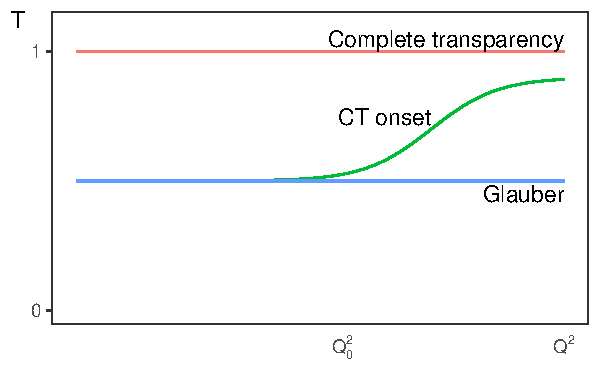
\includegraphics[width=0.8\textwidth]{chap1/CT_toy_prediction.pdf}
    \caption{
            An illustration of the $Q^2$ dependence of nuclear transparency $T$
            for three scenarios.
            The blue line illustrates the prediction of the Glauber model,
            which has constant $T$ as $Q^2$ increases.
            The red line illustrates that for full color transparency, $T=1$;
            in this scenario there are no final state interactions between the
            ejected proton and the rest of the nucleus.
            The green line illustrates the scenario where the transparency
            begins to deviate from the Glauber prediction above an onset
            $Q_0^2$ and approach $T=1$ with increasing $Q^2$.
            }
    \label{fig:CT_toy_prediction}
\end{figure}

Previous measurements of nuclear transparency in quasielastic electron
scattering experiments have been consistent with the Glauber prediction.
The goal of this experiment was to extend the range of $Q^2$ studied
in quasielastic ${}^12C(e,e'p)$ scattering in hopes of observing the onset
of CT.
Data were taken in Hall C at the Thomas Jefferson National Accelerator Facility
in Newport News, VA, using the High Momentum Spectrometer (HMS) and new Super
High Momentum Spectrometer (SHMS) in coincidence.
Data were taken with carbon foil and liquid hydrogen targets over a range of
momentum transfer $Q^2$ from 8.0 to \SI{14.3}{\giga\electronvolt\squared}.


Chapter 2 contains an overview of theoretical considerations relevant to
the experiment and a brief history of previous experiments that studied color
transparency.
Chapters 3 and 4 describe the experimental apparatus and data analysis
procedure.
Chapter 5 contains the final measurements of nuclear transparency and missing
energy and momentum.
Chapter 6 is a conclusion and summary.
